\documentclass[portrait]{tikzposter}

%TODO: autres styles ?
%TODO: logos
%TODO: nullfont ?  Dès le début de l'usage de tikzposter !
%TODO: font subst TS1/aer/m/n, cf \textbullet dans itemize

\definelayouttheme{MyBoard}{
    \usecolorstyle[colorPalette=BlueGrayOrange]{Spain}
    \usebackgroundstyle{Default}
    \usetitlestyle{Default}
    \useblockstyle{Basic}
    \useinnerblockstyle{Envelope}
    \usenotestyle{Sticky}
}

\usetheme{MyBoard}
\colorlet{backgroundcolor}{white}

%\usepackage{type1cm}
\usepackage{pgfplots}
\usepackage{tkz-euclide}% for geometry
\usepackage{tikz-qtree}
\usepackage{lipsum}% for dummy text
\usepackage{multicol}% for multiple columns
\setlength{\columnsep}{4cm}
\setlength{\columnseprule}{1mm}

\pgfplotsset{compat=1.18}

%\renewcommand*{\familydefault}{\sfdefault}% Let's have a sans serif font

\usetikzlibrary{lindenmayersystems,shadings}% gives us fractals
%\pgfdeclarelindenmayersystem{Koch curve}{
%  \rule{F -> F-F++F-F}}
%\pgfdeclarelindenmayersystem{Sierpinski triangle}{
%  \rule{F -> G-F-G}
%  \rule{G -> F+G+F}}
%\pgfdeclarelindenmayersystem{Fractal plant}{
%  \rule{X -> F-[[X]+X]+F[+FX]-X}
%  \rule{F -> FF}}
%\pgfdeclarelindenmayersystem{Hilbert curve}{
%  \rule{L -> +RF-LFL-FR+}
%  \rule{R -> -LF+RFR+FL-}}

\begin{document}
\title{\huge Curious recursive functions : Hostadter's G and after}
\author{Pierre Letouzey}
\institute{Picube, IRIF, UPC \& Inria \& CNRS}
\maketitle

\begin{columns}
  \column{.5}

  \block{Plotting G and after}{
\pgfplotsset{width=\linewidth}
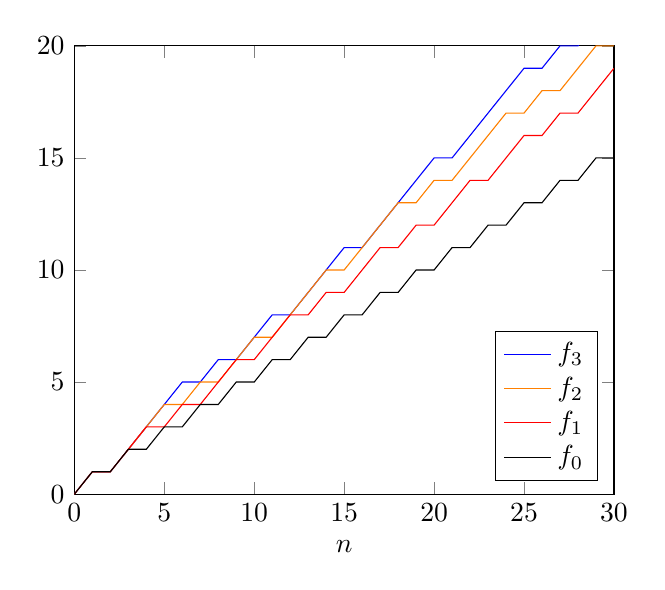
\begin{tikzpicture}[scale=1]
  \begin{axis}[
    xmin=0,xmax=30,ymin=0,ymax=20,samples=31,
    xlabel=$n$, legend pos=south east
  ]

    \addplot [mark=.,color=blue] coordinates {
(0, 0) (1, 1) (2, 1) (3, 2) (4, 3) (5, 4) (6, 5) (7, 5) (8, 6)
 (9, 6) (10, 7) (11, 8) (12, 8) (13, 9) (14, 10) (15, 11) (16, 11)
 (17, 12) (18, 13) (19, 14) (20, 15) (21, 15) (22, 16) (23, 17)
 (24, 18) (25, 19) (26, 19) (27, 20) (28, 20) (29, 21) (30, 22)};
 \addlegendentry{$f_3$}
    \addplot [mark=.,color=orange] coordinates {
(0, 0) (1, 1) (2, 1) (3, 2) (4, 3) (5, 4) (6, 4) (7, 5) (8, 5)
 (9, 6) (10, 7) (11, 7) (12, 8) (13, 9) (14, 10) (15, 10) (16, 11)
 (17, 12) (18, 13) (19, 13) (20, 14) (21, 14) (22, 15) (23, 16)
 (24, 17) (25, 17) (26, 18) (27, 18) (28, 19) (29, 20) (30, 20) };
 \addlegendentry{$f_2$}
 \addplot+[mark=.,domain=0:30,color=red]
 {floor((x+1) * 0.618033988749894903)};
 \addlegendentry{$f_1$}
 \addplot+[mark=.,domain=0:30] {ceil(x/2)};
 \addlegendentry{$f_0$}
 \end{axis}
\end{tikzpicture}
}%block

\block{The G tree}{

\begin{tikzpicture}[grow'=up,level distance=2cm]
\Tree
 [.1 [.2 [.3
       [.4 [.6 [.9 [.14 22 23 ] [.15 24 ] ]
               [.10 [.16 25 26 ]]]
           [.7 [.11 [.17 27 28 ] [.18 29 ]]]]
       [.5 [.8 [.12 [.19 30 31 ] [.20 32 ]]
               [.13 [.21 33 34 ]]]]]]]
\end{tikzpicture}
%TODO : et H ? et motifs d'arbres ?
}%block

\block{Fractal}{

\includegraphics[width=\linewidth]{fractal.png}

}%block



  \column{.5}
  \begin{subcolumns}
    \subcolumn{.5}
    \block{Mathematics}{
      Bla Bla
%%      Take a coffee, then:
%%       \vspace{1.4cm}
%%       \coloredbox{\begin{itemize}
%%         \item State
%%         \item Proof
%%         \item Write in \LaTeX
%%       \end{itemize}}
%%       \vspace{1.4cm}
%%       \innerblock{Integral approximation}{
%%         \[
%%           \int_a^b f(x) dx \approx (b-a)
%%             \sum_{i=0}^n w_i f(x_i)
%%         \]
%%       }
    }%block
     \note[targetoffsetx = 4.5cm, targetoffsety = -5cm,
       angle = -30, connection, width=10cm]{\Large Weight function}
    \subcolumn{.5}
    \block{Geometry}{
    %\vspace{-3cm}
    %\centering
%%     \begin{tikzpicture}[scale=1]
%%       \tkzDefPoint(0,0){A}
%%       \tkzDefPoint(4,1){B}
%%       \tkzInterCC(A,B)(B,A)
%%       \tkzGetPoints{C}{D}
%%       \tkzDrawPolygon(A,B,C)
%%       \tkzDrawPoints(A,B,C,D)
%%       \tkzLabelPoints[below left](A)
%%       \tkzLabelPoints(B,D)
%%       \tkzLabelPoint[above](C){$C$}
%%       \tkzDrawCircle[dotted](A,B)
%%       \tkzDrawCircle[dotted](B,A)
%%       \tkzCompass[color=red, very thick](A,C)
%%       \tkzCompass[color=red, very thick](B,C)
%%       \tkzCompass[color=red, very thick](A,D)
%%       \tkzCompass[color=red, very thick](B,D)
%%       \tkzDrawArc[fill=blue!10,thick](A,B)(C)
%%       \tkzDrawArc[fill=blue!10,thick](B,C)(A)
%%       \tkzDrawArc[fill=blue!10,thick](C,A)(B)
%%       \tkzInterLC(A,B)(B,A)
%%       \tkzGetPoints{F}{E}
%%       \tkzDrawPoints(E)
%%       \tkzLabelPoints(E)
%%       \tkzDrawPolygon(A,E,D)
%%       \tkzMarkAngles[fill=yellow,opacity=0.5](D,A,E A,E,D)
%%       \tkzMarkRightAngle[size=0.65,fill=red,opacity=0.5](A,D,E)
%%       \tkzLabelAngle[pos=0.7](D,A,E){\small$\alpha$}
%%       \tkzLabelAngle[pos=0.8](A,E,D){\small$\beta$}
%%       \tkzLabelAngle[pos=0.5,xshift=-1.4mm](A,D,D){\small$90^\circ$}
%%       \tkzLabelSegment[below=0.6cm,align=center,font=\small](A,B){Reuleaux\\triangle}
%%       \tkzLabelSegment[above right,sloped,font=\small](A,E){hypotenuse}
%%       \tkzLabelSegment[below,sloped,font=\small](D,E){opposite}
%%       \tkzLabelSegment[below,sloped,font=\small](A,D){adjacent}
%%       \tkzLabelSegment[below right=4cm,font=\small](A,E){Thales circle}
%%     \end{tikzpicture}
  }
  \end{subcolumns}
  \block{Fractals in \LaTeX}{
%    \lipsum[1]
    %\image[\LaTeX\ workflow]{flowchart}% if external
%%     \tikz\shadedraw[shading=color wheel,scale=2]
%%       [l-system={Koch curve, step=2pt, angle=60, axiom=F++F++F, order=4}]
%%         lindenmayer system -- cycle;\hfill
%%     \tikz\shadedraw [top color=white, bottom color=blue!80,scale=3,
%%       draw=blue!80!black] [l-system={Sierpinski triangle, step=2pt,
%%       angle=60, axiom=F, order=7}] lindenmayer system -- cycle;\hfill
%%     \tikz\shadedraw [bottom color=white, top color=red!80,scale=3,
%%       draw=red!80!black][l-system={Hilbert curve, axiom=L, order=4,
%%       step=8pt, angle=90}] lindenmayer system; \hfill
%%     \tikz\draw [green!50!black, rotate=90,scale=2]
%%       [l-system={Fractal plant, axiom=X, order=5, step=2pt, angle=25}]
%%       lindenmayer system;\hfill
%    \tikz\shade[shading=Mandelbrot set] (0,0) rectangle (15,15);
  }

%%   \block{Plotting functions}{
%%     %\image{plot}% if you would like to include an external image
%%     \pgfplotsset{width=\linewidth}
%%     \begin{tikzpicture}
%%       \begin{axis} [
%%         title = {$f(x,y) = \sin(x)\sin(y)$},
%%         xtick = {0,90,...,360},
%%         ytick = {90,180,...,360},
%%         xlabel = $x$, ylabel = $y$,
%%         ticklabel style = {font = \scriptsize},
%%         grid
%%       ]
%%       \addplot3 [surf, domain=0:360, samples=15]% raise samples if desired
%%         { sin(x)*sin(y) };
%%       \end{axis}
%%     \end{tikzpicture}
%% %    \lipsum[4]
%%   }
\end{columns}

%\block{Conclusion and outlook}{
%  \begin{multicols}{4}
%    \lipsum[1-2]
%  \end{multicols}
%}
\end{document}
